% title: Program optimization as a feedback loop
% description: A transformed program takes parameters, examples, and targets, and computes loss and parameter feedback. An update rule uses the feedback to revise the parameters, which return to the program on the next iteration. The optimization method supplies the update rule.
\documentclass[tikz,border=5pt]{standalone}
\usetikzlibrary{arrows.meta,calc,shapes.geometric}
\definecolor{numeric}{HTML}{4477AA}
\definecolor{textual}{HTML}{AA4499}

\tikzset{
    box/.style={draw, line width=0.8pt, minimum height=0.8cm,
                minimum width=1.8cm, inner sep=6pt, align=center},
    ir/.style={box},
    flow/.style={-{Stealth[length=5pt]}, line width=0.9pt},
    feedback/.style={flow, dashed},
    note/.style={font=\small, align=center},
    choice/.style={diamond, draw, line width=0.8pt,
                   aspect=2, inner sep=2pt, align=center},
}

\newcommand{\irframe}[2]{
    \draw[line width=0.8pt] #1 rectangle #2;
}

\newcommand{\transformarrow}[4][above]{
    \draw[flow] (#2) -- node[#1=6pt,note] {#4} (#3);
}


\begin{document}
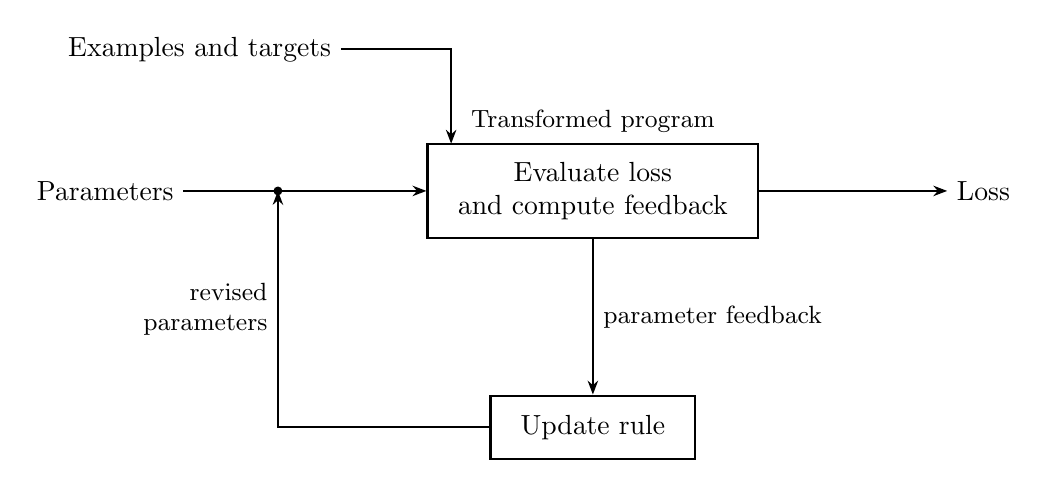
\begin{tikzpicture}

    \node[ir, minimum width=4.2cm, minimum height=1.2cm,
          label={[note]above:Transformed program}] (program) at (6,0)
        {Evaluate loss\\and compute feedback};
    \node[anchor=east] (parameters) at (0.8,0) {Parameters};
    \node[anchor=east] (data) at (2.8,1.8) {Examples and targets};
    \node[anchor=west] (loss) at (10.5,0) {Loss};
    \node[box, minimum width=2.6cm] (update) at (6,-3) {Update rule};

    \draw[flow] (parameters.east) -- (program.west);
    \draw[flow] (data.east) -| (4.2,0.6);
    \draw[flow] (program.east) -- (loss.west);
    \draw[flow] (program.south) -- node[right,note] {parameter feedback} (update.north);
    \draw[flow] (update.west) -- (2,-3)
        -- node[left,note,align=right] {revised\\parameters} (2,0);
    \fill (2,0) circle (1.6pt);

\end{tikzpicture}
\end{document}
